\section{Más funcionalidades útiles}
\frame
{
\frametitle{Más funcionalidades útiles}
\begin{center}
 
\includegraphics[height=7cm]{imgs/koala.jpg} 
\end{center}
}

\frame
{
\frametitle{pull}
Utilizándolo sin ningún parámetro adicional -\textbf{git pull origin master}- funciona igual que un \textit{update} en Subversion. Es decir, se trae los cambios y hace \textit{merge}. Si le pasamos el parámetro \textit{-{}-rebase}, funciona como un \textit{rebase}.

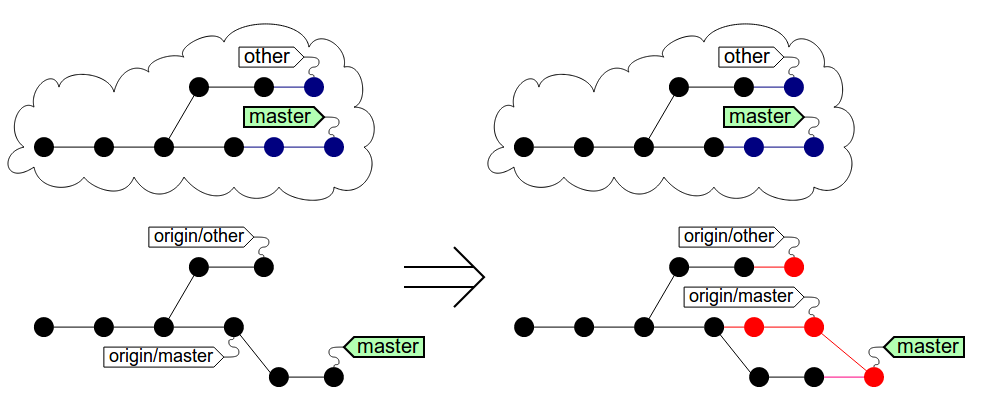
\includegraphics[height=5cm]{imgs/pull.png} 
}

\begin{frame}[fragile]
\frametitle{ignore}
El fichero \textit{.gitignore} se suele colocar en la raíz del proyecto y el contenido suele ser un listado de elementos que no queremos que sean reconocidos como ficheros del repositorio.
\footnotesize
\begin{verbatim}
neonigma@hyperion:~/things/taller-git$ cat .gitignore 
*.aux
*.bbl
*.log
*.backup
*.toc
*.dvi
*.out
neonigma@hyperion:~/things/taller-git$ git log principal.aux
neonigma@hyperion:~/things/taller-git$ 
\end{verbatim}
\end{frame}

\frame
{
\frametitle{update-index}
El comando update-index -{}-assume-unchanged se utiliza para ficheros que accidentalmente se han \textit{comiteado} (y probablemente \textit{pusheado}) y no queremos tener en cuenta los cambios producidos en estos ficheros, ya que lo veremos como modificados en la etapa II (listo para \textit{comitear}).
}

\frame
{
\frametitle{revert}
  Este comando deshace un único commit aplicando el parche con la diferencia como un nuevo commit. Ejemplo: git \textbf{revert} HEAD
 \begin{tabular}{p{4cm}|p{4cm}}\\
    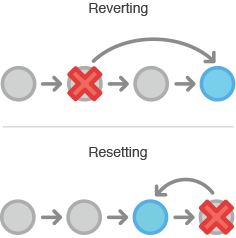
\includegraphics[height=4cm]{imgs/revert-vs-reset.png}&
    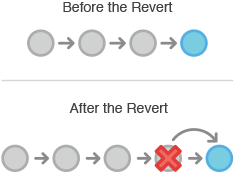
\includegraphics[height=3.5cm]{imgs/revert-sample.png}\\
 \end{tabular}

 Este comando no destruye la historia ni diverge las ramas \textit{master}. Ejemplo pack commits: git \textbf{revert} master\textasciitilde2..master
}

\frame
{
\frametitle{soft reset}
 El comando git reset -{}-soft <hash> mueve el puntero de la cabeza al hash del commit que le indiquemos.\\
 \begin{center}
    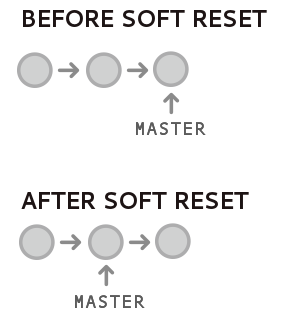
\includegraphics[height=4cm]{imgs/soft-reset.png}
 \end{center}
}

\frame
{
\frametitle{hard reset}
 El comando git reset -{}-hard <hash> mueve el puntero de la cabeza al hash del commit que le indiquemos y \textbf{destruye} toda la historia hasta dicho hash.\\
 \begin{center}
    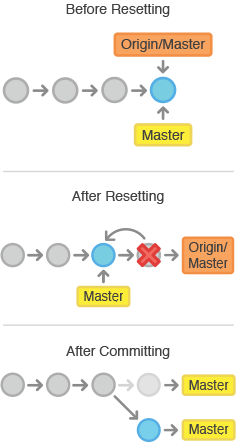
\includegraphics[height=6cm]{imgs/reset-hard.png}
 \end{center}
}

\section{Algo más avanzado}
\frame
{
\frametitle{Algo más avanzado}
\begin{center}
  
\includegraphics[height=7.5cm]{imgs/noidea.jpg}
\end{center}
}

\frame
{
\frametitle{stash}
 Se utiliza para \textit{aparcar} temporalmente los cambios actuales antes de ser comiteados. El comando se escribe únicamente git \textbf{stash}.
 \begin{framed}
 \$ git \textbf{stash} list\\
 stash@\{0\}: WIP on master: 049d078 added the index file\\
 stash@\{1\}: WIP on master: c264051... Revert added file\_size\\
 stash@\{2\}: WIP on master: 21d80a5... added number to log
 \end{framed}
 
 Recuperamos los cambios con el comando git \textbf{stash} apply <id>
}

\frame
{
\frametitle{format-patch}
 Se utiliza para generar parches que se entregarán a mantenedores de repositorios que no aceptan \textit{pull requests}.\\ \vspace{0.2cm}
 Un parche se genera con el comando git \textbf{format-patch} -{}-stdout \textit{<hash o rango de hashes>}. Esto genera tantos ficheros con parches como commits se hayan introducido como parámetro.\\ \vspace{0.2cm}
 Para aplicar los parches, se utiliza el comando git \textbf{am} -{}-signoff < \textit{file.patch}
}

\frame
{
\frametitle{squash}
 Se utiliza dentro de lo que se llama el \textit{rebase interactivo}, para unir varios commits en uno solo antes de entregarlos al repositorio remoto. El proceso sería:
 \begin{itemize}
  \item Comiteamos tantas veces como queramos: git commit -m ``mensaje''
  \item Si por ejemplo hemos hecho 2 commits, ejecutamos el rebase interactivo con: git \textbf{rebase} -i HEAD\textasciitilde2\\ \vspace{0.2cm}
  \footnotesize
   pick 4ca2acc commit file1\\
   pick 7b36971 commit file2\\
   
   \# rebase 41a72e6..7b36971 onto 41a72e6\\
   \#\\
   \# commands:\\
   \#  p, pick = use commit\\
   \#  r, reword = use commit, but edit the commit message\\
   \#  e, edit = use commit, but stop for amending\\
   \#  s, squash = use commit, but meld into previous commit\\
   \#  f, fixup = like ``squash'', but discard this commit's log message\\
   \#  x, exec = run command (the rest of the line) using shell
\end{itemize}
}

\frame
{
\frametitle{cherry-pick}
 \begin{itemize}
  \item Permite incorporar commits individuales a tu rama de trabajo
  \item El commit procederá de otra rama cualquiera
  \item La sintaxis: git \textbf{cherry-pick} <hash\_commit>
  \item La ventaja de esto es aprovechar funcionalidades comiteadas por otros miembros del equipo
  \item Si la recuperación del commit trae problemas de mezclado, se puede abortar esta recuperación con git \textbf{cherry-pick} -{}-abort
 \end{itemize}
}

\frame
{
\frametitle{reflog}
 \begin{itemize}
  \item Con git \textbf{log} vemos todos los commits realizados (historia)
  \item git \textbf{reflog} nos permite revisar todas las \textbf{acciones} realizadas
  \item Se puede utilizar para recuperar commits o ramas perdidas al utilizar git \textbf{reset}
  \item Los commits reseteados están disponibles durante 30 días, y los normales, durante 90 días
  \item[] \footnotesize 
	neonigma@hyperion:~/things/taller-git\$ git reflog\\
	abec02f HEAD@{0}: merge foo: Merge made by recursive.\\
	9bdbd83 HEAD@{1}: 9bdbd83: updating HEAD\\
	2d90ece HEAD@{2}: merge foo: Fast-forward\\
	9bdbd83 HEAD@{3}: checkout: moving from foo to master\\
	2d90ece HEAD@{4}: commit: hello\\
	9bdbd83 HEAD@{5}: checkout: moving from master to foo
\end{itemize}
}

\frame
{
\frametitle{submodules}
 \begin{itemize}
  \item submodules permite \textit{linkar} un repositorio dentro de otro
  \item Es una funcionalidad amada y odiada a partes iguales, por sus fuertes ventajas y desventajas
  \item Otras alternativas pasan por usar \textbf{subtree}, \textbf{gitslave} o \textbf{repo}
  \item Submodules es usado por:
    \begin{center}
      $\vcenter{\hbox{
\includegraphics[height=1.25in,width=1.5in]{imgs/gecos.png}}}$
      $\vcenter{\hbox{
\includegraphics[height=1.25in]{imgs/gnome.png}}}$
      $\vcenter{\hbox{
\includegraphics[height=1.25in]{imgs/android.png}}}$
    \end{center}
 \end{itemize}
}

\frame
{
\frametitle{submodules}
 \begin{itemize}
 \item Añadir un repositorio git como submódulo
  \begin{itemize}
    \item git \textbf{submodule} add [-b master] git@bitbucket.org:jialvarez/testproject.git
    \item git \textbf{commit} -m ``Añadimos submódulo testproject''
    \item git \textbf{push} <remote> <branch>
  \end{itemize}

 \item A partir de aquí el trabajo con el submódulo sería de manera normal, como un repositorio git cualquiera
 \item Tras actualizar el submódulo (add + commit + push), debemos actualizar también la referencia del padre de la misma manera
 \item ¡¡¡¡¡¡CUIDADO!!!!!! 
  \begin{itemize}
    \item Si hacemos \textit{push} en el proyecto padre y no en el proyecto hijo, el siguiente que haga un \textit{clone} del proyecto, no podrá descargarse todo el código al faltarle referencias
    \item Si no pusheamos el hijo y hacemos un par de commits, y luego tratamos de actualizar el padre con git submodule update, dejamos al hijo en DETACHED mode (sin ramas)
  \end{itemize}
 \end{itemize}
}

\frame
{
\frametitle{submodules}
 \begin{itemize}
 \item Descargar / actualizar repositorio conteniendo submódulos
  \begin{itemize}
   \item git \textbf{clone} git@bitbucket.org:jialvarez/testproject.git
   \item git \textbf{submodule} init
   \item git \textbf{submodule} update
  \end{itemize}

 \item Para hacer un barrido por todos los módulos y actualizarlos: \\git \textbf{submodule} foreach git pull origin master
 \item Para borrar un submódulo:
  \begin{itemize}
   \item Se eliminan sus líneas de configuración del fichero .gitmodules
   \item Se eliminan sus líneas de configuración del fichero .git/config
   \item Se ejecuta: git \textbf{rm} -{}-cached <path/to/submodule>
  \end{itemize}

  \item submodules es parte del \textit{core} de git y está disponible para todos los SO y bien integrado en GUIs
 \end{itemize}
}

\frame
{
\frametitle{lolcommits}
 \begin{itemize}
  \item Te permite tomar una foto desde la Webcam de manera automática cada vez que haces git commit
  \item Puede descargarse aquí: \url{http://mroth.github.io/lolcommits/}
  \item Tiene una lista de plugins para cambiar el vocabulario de commits, subir automáticamente las imágenes a un servidor, tuitear, etc.
  \item Se pueden hacer gif animados con las imágenes tomadas: \url{http://nacho-alvarez.es/descargas/myimage.gif}
  \item En Linux y Mac OS X es ultrasencillo de instalar, en Windows algo más complejo
  \item Para habililitar lolcommits en un repositorio git, sólo hay que escribir \textbf{lolcommits} -{}-enable
  \item Si queremos ver la última imagen: \textbf{lolcommits} -{}-last , si queremos abrir la carpeta: \textbf{lolcommits} -{}-browse
 \end{itemize}
}